\section{Sprites}

February 25, 2019  Victor Trucco

The Spectrum Next has a hardware sprite system with the following
characteristics:

\begin{itemize}
\item Total of 128 sprites
\item Display surface is $320\times256$ overlapping the ULA screen by
  32 pixels on each side
\item Minimum of 100 sprites per scanline*
\item Choice of 512 colours for each pixel
\item Site of each sprite is $16\times16$ pixels but sprites can be
  magnified $2\times$, $4\times$ or $8\times$ horizontally and
  vertically
\item Sprites can be mirrored and rotated
\item Sprites can be grouped together to form larger sprites under the
  control of a single anchor
\item A 16K pattern memory can contain 64 8-bit sprite images or 128
  4-bit sprite images and combinations in-between
\item A per sprite palette offset allows sprites to share images but
  colour them differently
\item A nextreg interface allows the copper to move sprites during the
  video frame
\end{itemize}

*A minimum of 100 $16\times16$ sprites is guaranteed to be displayed
in any scanline. Any additional sprites will not be displayed with the
hardware ensuring sprites are not partially plotted.

The actual limit is determined by how many 28MHz clock cycles there
are in a scanline. The sprite hardware is able to plot one pixel cycle
and uses one cycle to qualify each sprite. Since the number of cycles
there are in a scanline varies with video timing (HDMI, VGA), the
number of pixels that can be plotted also varies but the minimum will
be 1600 pixels per line including overhead cycles needed to qualify
100 sprites. Since sprites magified horizontally involve plotting more
pixels, $2\times$, $4\times$, and $8\times$ sprites will take more
cycles to plot and the presence of these sprites in a line will reduce
the total number of sprites that can be plotted.

\subsection{Sprite Patterns}
Sprite patterns are the images that each sprite can take on. The
images are stored in a 16K memory internal to the FPGA and are
identified by pattern number. A particular sprite chooses a pattern by
storing a pattern number in its attributes.

All sprites are $16\times16$ pixels in size but the come in two
flavours: 4-bit and 8-bit. The bit width describes how many bits are
used to code the colour of each pixel.

An 8-bit sprite uses a full byte to colour each of its pixels so that
each pixel can be one of 256 colours. In this case, a $16\times16$
sprite requires 256 bytes of pattern memory to store its image.

A 4-bit sprite uses a nibble to colour each of its pixels so that each
pixel can be one of 16 colours. In this case, a $16\times16$ sprite
requires just 128 bytes of pattern memory to store its image.

The 16K pattern memory can contain any combination of these images,
whether they are 128 bytes or 256 bytes and their locations in the
pattern memory are described by a pattern number. This pattern number
is 7 bits with bits named as follows:

\paragraph{Pattern Number}
\begin{verbatim}
N5 N4 N3 N2 N1 N0 N6
\end{verbatim}
N6, despite the name, is the least significant bit.

This 7-bit pattern number can identify 128 patterns in the 16k pattern
memory, each of which are 128 bytes in size. The full 7-bits are
therefore used for 4-bit sprites.

For 8-bit sprites, N6=0 always. The remaining 6 bits can identify 64
patterns, each of which is 256 bytes in size.

The N5:N0,N6 bits are stored in a particular sprite’s attributes to
identify which image a sprite uses.

\subparagraph{8-Bit Sprite Patterns}

The $16\times16$ pixel image uses 8-bits for each pixel so that each
pixel can be one of 256 colours. One colour indicates transparency and
this is programmed into the Sprite Transparency Index register
(nextreg \$4B). By default the transparent value is \$E3.

As an example of an 8-bit sprite, let’s have a look at figure 1.1.

\begin{figure}\centering
  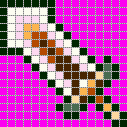
\includegraphics{video/sprite_1.png}
  \caption{Pattern Example}
\end{figure}

Using the default palette, which is initialised with RGB332 colours
from 0-255, the hexadecimal values for this pattern arranged in a
$16\times16$ array are shown below:

\begin{verbatim}
04040404040404E3E3E3E3E3E3E3E3E3
04FFFFFFFFFF04E3E3E3E3E3E3E3E3E3
04FFFBFBFBFF04E3E3E3E3E3E3E3E3E3
04FFFBF5F5FBFF04E3E3E3E3E3E3E3E3
04FFFBF5A8A8FBFF04E3E3E3E3E3E3E3
04FFFFFBA844A8FBFF04E3E3E3E3E3E3
040404FFFBA844A8FBFF04E3E3E3E3E3
E3E3E304FFFBA84444FBFF04E304E3E3
E3E3E3E304FFFB444444FBFF044D04E3
E3E3E3E3E304FFFB44444444FA4D04E3
E3E3E3E3E3E304FFFB44FFF54404E3E3
E3E3E3E3E3E3E304FF44F5A804E3E3E3
E3E3E3E3E3E3E3E304FA4404A804E3E3
E3E3E3E3E3E3E3044D4D04E304F504E3
E3E3E3E3E3E3E3E30404E3E3E304FA04
E3E3E3E3E3E3E3E3E3E3E3E3E3E30404

\end{verbatim}
Here \$E3 is used as the transparent index.

These 256 bytes would be stored in pattern memory in left to right,
top to bottom order.

\subparagraph{4-Bit Sprite Patterns}

The $16\times16$ pixel image uses 4-bits for each pixel so that each
pixel can be one of 16 colours. One colour indicates transparency and
this is programmed into the lower 4-bits of the Sprite Transparency
Index register (nextreg \$4B). By default the transparency value is
\$3. Note that the same register is shared with 8-bit patterns to
identify the transparent index.

Since each pixel only occupies 4-bits, two pixels are stored in each
byte. The leftmost pixel is stored in the upper 4-bits and the
rightmost pixel is stored in the lower 4-bits.

As an example we will use the same sprite image as was given in the
8-bit pattern example. Here only the lower 4 bits of each pixel is
retained to confine each pixel’s color to 4-bits:

\begin{verbatim}
4444444333333333
4FFFFF4333333333
4FBBBF4333333333
4FB55BF433333333
4FB588BF43333333
4FFB848BF4333333
444FB848BF433333
3334FB844BF43433
33334FB444BF4D43
333334FB4444AD43
3333334FB4F54433
33333334F4584333
333333334A448433
33333334DD434543
33333333443334A4
3333333333333344
\end{verbatim}

\$3 is used as the transparent index.

These 128 bytes would be stored in pattern memory in left to right,
top to bottom order.

The actual colour that will appear on screen will depend on the
palette, described below. The default palette will not likely generate
suitable colours for 4-bit sprites.

\subsection{Sprite Palette}
Each pixel of a sprite image is 8-bit for 8-bit patterns or 4-bit for
4-bit patterns. The pixel value is known as a pixel colour index. This
colour index is combined with the sprite’s palette offset. The palette
offset is a 4-bit value added to the top 4-bits of the pixel colour
index. The purpose of the palette offset is to allow a sprite to
change the colour of an image.

The final sprite colour index generated by the sprite hardware is then
the sum of the pixel index and the 4-bit palette offset. In pictures
using binary math:

\begin{verbatim}
8-bit Sprite
PPPP0000
+ IIIIIIII
----------
SSSSSSSS

4-bit Sprite
PPPP0000
+ 0000IIII
----------
SSSSSSSS = PPPPIIII
\end{verbatim}

Where “PPPP” is the 4-bit palette offset from the sprite’s attributes
and the “I”s represent the pixel value from the sprite pattern. The
final sprite index is represented by the 8-bit value “SSSSSSSS”.

For 4-bit sprites the palette offset can be thought of as selecting
one of 16 different 16-colour palettes.

This final 8-bit sprite index is then passed through the sprite
palette which acts like a lookup table that returns the 9-bit RGB333
colour associated with the sprite index.

At power up, the sprite palette is initialized such that the sprite
index passes through unchanged and is therefore interpretted as an
RGB332 colour. The missing third blue bit is generated as the logical
OR of the two other blue bits. In short, for 8-bit sprites, the sprite
index also acts like the colour when using the default palette.

\subsection{Sprite Attributes}
A sprite’s attributes is a list of properties that determine how and
where the sprite is drawn.

Each sprite is described by either 4 or 5 attribute bytes listed
below:

Sprite Attribute 0
\begin{verbatim}
X X X X X X X X
\end{verbatim}
The least significant eight bits of the sprite’s X coordinate. The
ninth bit is found in sprite attribute 2.

Sprite Attribute 1
\begin{verbatim}
Y Y Y Y Y Y Y Y
\end{verbatim}
The least significant eight bits of the sprite’s Y coordinate. The
ninth bit is optional and is found in attribute 4.

Sprite Attribute 2
\begin{verbatim}
P P P P XM YM R X8/PR
\end{verbatim}
P = 4-bit Palette Offset

XM = 1 to mirror the sprite image horizontally

YM = 1 to mirror the sprite image vertically

R = 1 to rotate the sprite image 90 degrees clockwise

X8 = Ninth bit of the sprite’s X coordinate

PR = 1 to indicate P is relative to the anchor’s palette offset
(relative sprites only)

Rotation is applied before mirroring.

Relative sprites, described below, replace X8 with PR.

\begin{figure}\centering
  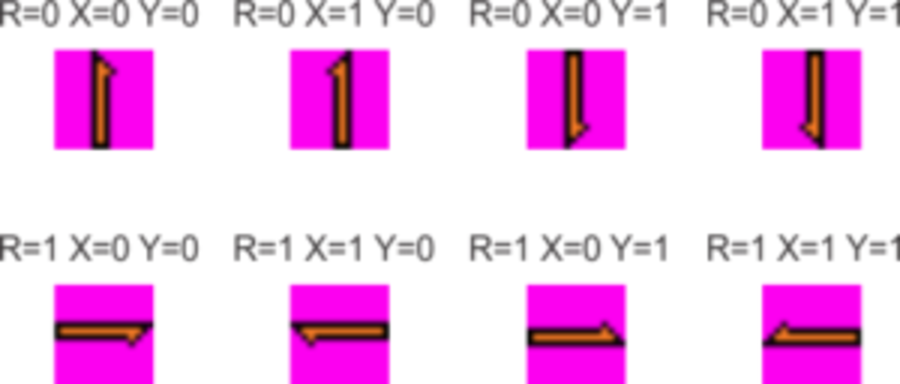
\includegraphics{video/flags.png}
  \caption{All Rotate and Mirror Flags}
\end{figure}

Sprite Attribute 3
\begin{verbatim}
V E N5 N4 N3 N2 N1 N0
\end{verbatim}
V = 1 to make the sprite visible

E = 1 to enable attribute byte 4

N = Sprite pattern to use 0-63

If E=0, the sprite is fully described by sprite attributes 0-3. The
sprite pattern is an 8-bit one identified by pattern N=0-63. The
sprite is an anchor and cannot be made relative. The sprite is
displayed as if sprite attribute 4 is zero.

If E=1, the sprite is further described by sprite attribute 4.

Sprite Attribute 4
\begin{enumerate}[A.]
\item Extended Anchor Sprite
\begin{verbatim}
H N6 T X X Y Y Y8
\end{verbatim}
H = 1 if the sprite pattern is 4-bit

N6 = 7th pattern bit if the sprite pattern is 4-bit

T = 0 if relative sprites are composite type else 1 for unified type

XX = Magnification in the X direction (00 = $1\times$, 01 = $2\times$,
10 = $4\times4$, 11 = $8\times$)

YY = Magnification in the Y direction (00 = $1\times$, 01 = $2\times$,
10 = $4\times$, 11 = $8\times$)

Y8 = Ninth bit of the sprite’s Y coordinate

{H,N6} must not equal {0,1} as this combination is used to indicate a
relative sprite.

\item Relative Sprite, Composite Type
\begin{verbatim}
0 1 N6 X X Y Y PO
\end{verbatim}
N6 = 7th pattern bit if the sprite pattern is 4-bit

XX = Magnification in the X direction (00 = $1\times$, 01 = $2\times$,
10 = $4\times$, 11 = $8\times$)

YY = Magnification in the Y direction (00 = $1\times$, 01 = $2\times$,
10 = $4\times$, 11 = $8\times$)

PO = 1 to indicate the sprite pattern number is relative to the
anchor’s

\item Relative Sprite, Unified Type
\begin{verbatim}
0 1 N6 0 0 0 0 PO
\end{verbatim}
N6 = 7th pattern bit if the sprite pattern is 4-bit

PO = 1 to indicate the sprite pattern number is relative to the
anchor’s
\end{enumerate}
The display surface for sprites is $320\times256$. The X coordinate of
the sprite is nine bits, ranging over 0-511, and the Y coordinate is
optionally nine bits again ranging over 0-511 or is eight bits ranging
over 0-255. The full extent 0-511 wraps on both axes, meaning a sprite
16 pixels wide plotted at X coordinate 511 would see its first pixel
not displayed (coordinate 511) and the following pixels displayed in
coordinates 0-14.

The full display area is visible in VGA. However, the HDMI display is
vertically shorter so the top eight pixel rows (Y = 0-7) and the
bottom eight pixel rows (Y = 248-255) will not be visible on an HDMI
display.

Sprites can be fully described by sprite attributes 0-3 if the E bit
in sprite attribute 3 is zero. These sprites are compatible with the
original sprite module from core versions prior to 2.00.26.

If the E bit is set then a fifth sprite attribute, sprite attribute 4,
becomes active. This attribute introduces scaling, 4-bit patterns, and
relative sprites. Scaling is self-explanatory and 4-bit patterns were
described in the last section. Relative sprites are described in the
next section.

\subsection{Relative Sprites}
Normal sprites (sprites that are not relative) are known as anchor
sprites. As the sprite module draws sprites in the order 0-127 (there
are 128 sprites), it internally stores characteristics of the last
anchor sprite seen. If following sprites are relative, they inherit
some of these characteristics, which allows relative sprites to have,
among other things, coordinates relative to the anchor. This means
moving the anchor sprite also causes its relatives to move with it.

There are two types of relative sprites supported known as “Composite
Sprites” and “Unified Sprites”. The type is determined by the anchor
in the T bit of sprite attribute 4.

\begin{enumerate}[A.]
\item Composite Sprites

  The sprite module records the following information from the anchor:
  \begin{itemize}
  \item Anchor.visible
  \item Anchor.Y
  \item Anchor.palette\_offset
  \item Anchor.N (pattern number)
  \item Anchor.H (indicates if the sprite uses 4-bit patterns)
  \end{itemize}
  These recorded items are not used by composite sprites:
  \begin{itemize}
  \item Anchor.rotate
  \item Anchor.xmirror
  \item Anchor.ymirror
  \item Anchor.xscale
  \item Anchor.yscale
  \end{itemize}
  The anchor determines if all its relative sprites use 4-bit patterns or not.
  
  The visibility of a particular relative sprite is the result of
  ANDing the anchor’s visibility with the relative sprite’s
  visibility. In other words, if the anchor is invisible then so are
  all its relatives.

  Relative sprites only have 8-bit X and Y coordinates (the ninth bits
  are taken for other purposes). These are signed offsets from the
  anchor’s X,Y coordinate. Moving the anchor moves all its relatives
  along with it.

  If the relative sprite has its PR bit set in sprite attribute 2,
  then the anchor’s palette offset is added to the relative sprite’s
  to determine the active palette offset for the relative
  sprite. Otherwise the relative sprite uses its own palette offset as
  usual.

  If the relative sprite has its PO bit set in sprite attribute 4,
  then the anchor’s pattern number is added to the relative sprite’s
  to determine the pattern used for display. Otherwise the relative
  sprite uses its own pattern number as usual. The intention is to
  supply a method to easily animate a large sprite by manipulating the
  pattern number in the anchor.

  A composite sprite is like a collection of independent sprites tied
  to an anchor.

\item Unified Sprites

  Unified sprites are a further extension of the
  composite type. The same information is recorded from the anchor and
  the same behaviour as described under composite sprites applies.

  The difference is the collection of anchor and relatives is treated
  as if it were a single $16\times16$ sprite. The anchor’s rotation,
  mirror, and scaling bits apply to all its relatives. Rotating the
  anchor causes all the relatives to rotate around the
  anchor. Mirroring the anchor causes the relatives to mirror around
  the anchor. The sprite hardware will automatically adjust X,Y coords
  and rotation, scaling and mirror bits of all relatives according to
  settings in the anchor.

  Unified sprites should be defined as if all its parts are
  $16\times16$ in size with the anchor controlling the look of the
  whole.

  A unified sprite is like a big version of an individual $16\times16$
  sprite controlled by the anchor.
\end{enumerate}

\subsection{Programming Sprites}

Sprites are created via three io registers and a nextreg interface.

Port \$303B (W)
\begin{verbatim}
X S S S S S S S
N6 X N N N N N N
\end{verbatim}
A write to this port has two effects.

One is it selects one of 128 sprites for writing sprite attributes via
port \$57.

The other is it selects one of 128 4-bit patterns in pattern memory
for writing sprite patterns via port \$5B. The N6 bit shown is the
least significant in the 7-bit pattern number and should always be
zero when selecting one of 64 8-bit patterns indicated by N.

Port \$57 (W)

Once a sprite is selected via port \$303B, its attributes can be
written to this port one byte after another. Sprites can have either
four or five attribute bytes and the internal attribute pointer will
move onto the next sprite after those four or five attribute bytes are
written. This means you can select a sprite via port \$303B and write
attributes for as many sequential sprites as desired. The attribute
pointer will roll over from sprite 127 to sprite 0.

Port \$5B (W)

Once a pattern number is selected via port \$303B, the 256-byte or
128-byte pattern can be written to this port. The internal pattern
pointer auto-increments after each write so as many sequential
patterns as desired can be written. The internal pattern pointer will
roll over from pattern 127 to pattern 0 (4-bit patterns) or from
pattern 63 to pattern 0 (8-bit patterns) automatically.

Port \$303B (R)

\begin{verbatim}
0 0 0 0 0 0 M C
\end{verbatim}
M = 1 if the maximum number of sprites per line was exceeded

C = 1 if any two displayed sprites collide on screen

Reading this port automatically resets the M and C bits.

Besides the i/o interface, there is a nextreg interface to sprite
attributes. The nextreg interface allows the copper to manipulate
sprites and grants the program random access to a sprite’s individual
attribute bytes.

(R/W) \$34 (52) $\Rightarrow$ Sprite Number

If the sprite number is in lockstep with io port \$303B (nextreg \$09
bit 4 is set)
\begin{itemize}
\item[] bits 7 = Pattern address offset (Add 128 to pattern address)
\item[] bits 6-0 = Sprite number 0-127, Pattern number 0-63
\end{itemize}
Selects which sprite has its attributes connected to the following registers.

Effectively performs an out to port \$303B with the same value

Otherwise
\begin{itemize}
\item[] bit 7 = Ignored
\item[] bits 6-0 = Sprite number 0-127
\end{itemize}
Selects which sprite has its attributes connected to the following registers.

Bit 7 always reads back as zero.

This nextreg can operate in two modes.

If nextreg \$09 bit 4 is set, then this register is kept in lockstep
with i/o port \$303B. A write to this nextreg is equivalent to a write
to port \$303B and vice versa. In this mode, the i/o interface and
nextreg interface are exactly equivalent.

If nextreg \$09 bit 4 is reset, then the nextreg interface is
decoupled from i/o port \$303B. This nextreg is used to select a
particular sprite 0-127 and this is completely independent from the
sprite selected for the i/o interface. This independence allows the
copper, for example, to manipulate different sprites than the cpu
using the i/o interface.

(W) \$35 (53) $\Rightarrow$ Sprite Attribute 0

(W) \$75 (117) $\Rightarrow$ Sprite Attribute 0 with automatic post
increment of Sprite Number
\begin{itemize}
\item[] bits 7-0 = LSB of X coordinate
\end{itemize}
A write to nextreg \$75 also increases the selected sprite in nextreg
\$34.

(W) \$36 (54) $\Rightarrow$ Sprite Attribute 1

(W) \$76 (118) $\Rightarrow$ Sprite Attribute 1 with automatic post
increment of Sprite Number
\begin{itemize}
\item[] bits 7-0 = LSB of Y coordinate
\end{itemize}
A write to nextreg \$76 also increases the selected sprite in nextreg
\$34.

(W) \$37 (55) $\Rightarrow$ Sprite Attribute 2

(W) \$77 (119) $\Rightarrow$ Sprite Attribute 2 with automatic post
increment of Sprite Number
\begin{itemize}
\item[] bits 7-4 = Palette offset added to top 4 bits of sprite colour
  index
\item[] bit 3 = X mirror
\item[] bit 2 = Y mirror
\item[] bit 1 = Rotate
\item[] bit 0 = MSB of X coordinate
\end{itemize}
A write to nextreg \$77 also increases the selected sprite in nextreg
\$34.

(W) \$38 (56) $\Rightarrow$ Sprite Attribute 3

(W) \$78 (120) $\Rightarrow$ Sprite Attribute 3 with automatic post
increment of Sprite Number
\begin{itemize}
\item[] bit 7 = Visible flag (1 = displayed)
\item[] bit 6 = Extended attribute (1 = Sprite Attribute 4 is active)
\item[] bits 5-0 = Pattern used by sprite (0-63)
\end{itemize}
A write to nextreg \$78 also increases the selected sprite in nextreg
\$34.

(W) \$39 (57) $\Rightarrow$ Sprite Attribute 4

(W) \$79 (121) $\Rightarrow$ Sprite Attribute 4 with automatic post
increment of Sprite Number

4-bit Sprites
\begin{itemize}
\item[] bit 7 = H (1 = sprite uses 4-bit patterns)
\item[] bit 6 = N6 (0 = use the first 128 bytes of the pattern else
  use the last 128 bytes)
\item[] bit 5 = 1 if relative sprites are composite, 0 if relative
  sprites are unified Scaling
\item[] bits 4-3 = X scaling (00 = 1x, 01 = 2x, 10 = 4x, 11 = 8x)
\item[] bits 2-1 = Y scaling (00 = 1x, 01 = 2x, 10 = 4x, 11 = 8x)
\item[] bit 0 = MSB of Y coordinate
\end{itemize}
A relative mode is enabled if H,N6 = 01. The byte format for relative
sprites is described above.

A write to nextreg \$79 also increases the selected sprite in nextreg
\$34.

\subsection{Global Control of Sprites}

The following nextreg are also of interest for sprites.

(R/W) \$09 (09) $\Rightarrow$ Peripheral 4 setting:
\begin{itemize}
\item[] bit 7 = Mono setting for AY 2 (1 = mono, 0 default)
\item[] bit 6 = Mono setting for AY 1 (1 = mono, 0 default)
\item[] bit 5 = Mono setting for AY 0 (1 = mono, 0 default)
\item[] bit 4 = Sprite id lockstep (1 = Nextreg \$34 and IO Port
  \$303B are in lockstep, 0 default)
\item[] bit 3 = Disables Kempston port (\$DF) if set
\item[] bit 2 = Disables divMMC ports (\$E3, \$E7, \$EB) if set
\item[] bits 1-0 = scanlines (0 after a PoR or Hard-reset)
  \begin{itemize}
  \item[] 00 = scanlines off
  \item[] 01 = scanlines 75\%
  \item[] 10 = scanlines 50\%
  \item[] 11 = scanlines 25\%
  \end{itemize}
\end{itemize}

Bit 4 determines if the i/o interface and nextreg interface operate in lockstep.

(R/W) \$15 (21) $\Rightarrow$ Sprite and Layers system
\begin{itemize}
\item[] bit 7 = LoRes mode, $128\times96\times256$ colours (1 =
  enabled)
\item[] bit 6 = Sprite priority (1 = sprite 0 on top, 0 = sprite 127
  on top)
\item[] bit 5 = Enable sprite clipping in over border mode (1 =
  enabled)
\item[] bits 4-2 = set layers priorities:

Reset default is 000, sprites over the Layer 2, over the ULA graphics
\begin{itemize}
\item[] 000 – S L U
\item[] 001 – L S U
\item[] 010 – S U L
\item[] 011 – L U S
\item[] 100 – U S L
\item[] 101 – U L S
\item[] 110 – S(U+L) ULA and Layer 2 combined, colours clamped to 7
\item[] 111 – S(U+L-5) ULA and Layer 2 combined, colours clamped to
  [0,7]
\end{itemize}
\item[] bit 1 = Over border (1 = yes)(Back to 0 after a reset)
\item[] bit 0 = Sprites visible (1 = visible)(Back to 0 after a reset)
\end{itemize}

Bit 0 must be set for sprites to be visible.

Bit 1 set allows sprites to be visible in the border area. When this
bit is reset, sprites will not display outside the $256\times192$ area
of the ULA display.

Bit 5 set enables clipping when sprites are visible in the border
area. If reset, no clipping is applied and sprites will be visible in
the full $320\times256$ space.

The sprite module draws sprites in the order 0-127 in each
scanline. Bit 6 determines whether sprite 0 is topmost or sprite 127
is topmost.

Bits 4:2 determine layer priority and how sprites overlay or are
obscured by other layers.

(R/W) \$19 (25) $\Rightarrow$ Clip Window Sprites
\begin{itemize}
\item[] bits 7-0 = Cood. of the clip window
  \begin{itemize}
  \item[] 1st write – X1 position
  \item[] 2nd write – X2 position
  \item[] 3rd write – Y1 position
  \item[] 4rd write – Y2 position
  \end{itemize}
\end{itemize}
The values are 0,255,0,191 after a Reset

Reads do not advance the clip position

When the clip window is enabled for sprites in “over border” mode, the
X coords are internally doubled and the clip window origin is moved to
the sprite origin inside the border.

Sprites will only be visible inside the clipping window. When not in
over-border mode (bit 1 of nextreg \$15) the clipping window is given
in ULA screen coordinates with 0,0 correspoding to the top left corner
of the ULA screen. In over-border mode, the clipping window’s origin
is moved to the sprite coordinate origin 32 pixels to the left and 32
pixels above the ULA screen origin.

Regardless, sprite position is always in sprite coordinates with 32,32
corresponding to the top left corner of the ULA screen.

(W) \$1C (28) $\Rightarrow$ Clip Window control
\begin{itemize}
\item[] bits 7-4 = Reserved, must be 0
\item[] bit 3 – reset the tilemap clip index
\item[] bit 2 – reset the ULA/LoRes clip index.
\item[] bit 1 – reset the sprite clip index.
\item[] bit 0 – reset the Layer 2 clip index.
\end{itemize}

Can be used to reset nextreg \$19.

(R/W) \$43 (67) $\Rightarrow$ Palette Control
\begin{itemize}
\item[] bit 7 = ‘1’ to disable palette write auto-increment.
\item[] bits 6-4 = Select palette for reading or writing:
  \begin{itemize}
  \item[] 000 = ULA first palette
  \item[] 100 = ULA second palette
  \item[] 001 = Layer 2 first palette
  \item[] 101 = Layer 2 second palette
  \item[] 010 = Sprites first palette
  \item[] 110 = Sprites second palette
  \item[] 011 = Tilemap first palette
  \item[] 111 = Tilemap second palette
  \end{itemize}
\item[] bit 3 = Select Sprites palette (0 = first palette, 1 = second
  palette)
\item[] bit 2 = Select Layer 2 palette (0 = first palette, 1 = second
  palette)
\item[] bit 1 = Select ULA palette (0 = first palette, 1 = second
  palette)
\item[] bit 0 = Enabe ULANext mode if 1. (0 after a reset)
\end{itemize}

Sprites have two associated palettes which can be selected in this nextreg.

(R/W) \$40 (64) $\Rightarrow$ Palette Index
\begin{itemize}
\item[] bits 7-0 = Select the palette index to change the associated
  colour.
\end{itemize}
For the ULA only, INKs are mapped to indices 0-7, Bright INKS to
indices 8-15, PAPERs to indices 16-23 and Bright PAPERs to indices
24-31.

In ULANext mode, INKs come from a subset of indices 0-127 and PAPERs
come from a subset of indices 128-255. The number of active indices
depends on the number of attribute bits assigned to INK and PAPER out
of the attribute byte.  The ULA always takes border colour from paper.

Select the starting palette index if writing the sprite palette.

Palette values can be written in either 8-bit or 9-bit form:

(R/W) \$41 (65) $\Rightarrow$ Palette Value (8 bit colour)
\begin{itemize}
\item[] bits 7-0 = Colour for the palette index selected by the register \$40.
\end{itemize}
(Format is RRRGGGBB – the lower blue bit of the 9-bit colour will be a
logical OR of blue bits 1 and 0 of this 8-bit value.)

After the write, the palette index is auto-incremented to the next
index if the auto-increment is enabled at reg \$43. Reads do not
auto-increment.

(R/W) \$44 (68) $\Rightarrow$ Palette Value (9 bit colour)

Two consecutive writes are needed to write the 9 bit colour
\begin{itemize}
\item[] 1st write:
  \begin{itemize}
  \item[] bits 7-0 = RRRGGGBB
  \end{itemize}
\item[] 2nd write.
  If writing a L2 palette
  \begin{itemize}
  \item[] bit 7 = 1 for L2 priority colour, 0 for normal

    Priority colour will always be on top even on an SLU priority
    arrangement. If you need the exact same colour on priority and non
    priority locations you will need to program the same colour twice
    changing bit 7 to 0 for the second colour
  \item[] bits 6-1 = Reserved, must be 0
  \item[] bit 0 = lsb B
  \end{itemize}
  
  If writing another palette
  \begin{itemize}
  \item[] bits 7-1 = Reserved, must be 0
  \item[] bit 0 = lsb B
  \end{itemize}
\end{itemize}


After the two consecutives writes the palette index is
auto-incremented if the auto-increment is enabled by reg \$43.

Reads only return the 2nd byte and do not auto-increment.

(R/W) \$4B (75) $\Rightarrow$ Transparency index for sprites
\begin{itemize}
\item[] bits 7-0 = Set the index value (\$E3 after reset)
\end{itemize}
For 4-bit sprites only the bottom 4-bits are relevant.

Determines the transparent colour index used for sprites.
